\documentclass{article}

\usepackage[final]{nips_2016}
\usepackage[utf8]{inputenc}
\usepackage[T1]{fontenc}
\usepackage{hyperref}
\usepackage{url}
\usepackage{booktabs}
\usepackage{amsfonts}
\usepackage{amsmath}
\usepackage{nicefrac}
\usepackage{microtype}
\usepackage{graphicx}
\usepackage{pgfplots}
\pgfplotsset{compat=1.13}
\setcitestyle{numbers,square,comma}

\title{Generating Clinical Texts from Conversation}

\author{
  Teppei Nakano \\
  Keio University School of Medicine \\
  Tokyo, Japan \\
  \texttt{keiohigh2nd@gmail.com}
}

\begin{document}

\maketitle

\begin{abstract}
Documenting an encounter is one of the most time-consuming parts of a clinician's
day, and the source material for that documentation---the spoken exchange between
clinician and patient---is largely discarded. We study the task of generating a
draft clinical note directly from the transcript of a doctor--patient conversation.
The task is a form of abstractive summarization with two distinguishing features:
the target is highly structured (chief complaint, history of present illness,
review of systems, assessment), and the salient tokens are rare, out-of-vocabulary
medical terms---drug names, dosages, and findings---that a purely generative
decoder tends to mangle. We adopt an attentional sequence-to-sequence model built
from bidirectional long short-term memory encoders and an LSTM decoder, and augment
it with a copy mechanism that lets the decoder point back to conversation tokens,
so that rare clinical terms are transcribed verbatim rather than hallucinated. On a
corpus of $12{,}148$ conversation--note pairs we find that copying improves ROUGE-L
from $31.4$ to $38.7$ and, more importantly for clinical use, raises the F1 of
correctly rendered medical concepts from $0.52$ to $0.71$. A blinded review by
clinicians rated $63\%$ of generated drafts as requiring only minor edits. We
analyze the remaining failure modes, which are dominated by errors of omission on
information stated only implicitly in the dialogue.
\end{abstract}

\section{Introduction}

Clinical documentation consumes an outsized share of clinician time and is a
leading contributor to burnout. Yet the raw material for a note---what was actually
said during the visit---is rich and, increasingly, capturable through ambient or
dictated speech. If a faithful draft note could be produced automatically from the
conversation, the clinician's role would shift from authoring to reviewing, a far
lighter task. We formalize and study this problem: given a transcript of a
doctor--patient conversation, generate the corresponding clinical note.

Framed as a sequence transduction problem, note generation resembles abstractive
summarization, for which attentional encoder--decoder networks had by 2016 become
the dominant approach \citep{Bahdanau2015,Rush2015,Nallapati2016}. But two
properties of the clinical setting make a direct application inadequate. First, the
target is not free prose but a semi-structured document whose sections follow a
stereotyped order; a good model should respect this structure. Second, and more
consequentially, the information a note must get exactly right is carried by rare
tokens: medication names, numeric doses, laboratory values, and specific findings.
These are precisely the tokens a fixed-vocabulary decoder handles worst, either
emitting an \texttt{<unk>} symbol or substituting a frequent but wrong term. In
medicine, ``metoprolol'' rendered as ``metformin'' is not a small error.

Both difficulties point to the same remedy: the decoder should be able to
\emph{copy} spans directly from the source conversation. We therefore build on the
attentional sequence-to-sequence architecture and add a copy mechanism
\citep{Gu2016,Gulcehre2016} that, at each decoding step, chooses between generating
a word from the vocabulary and pointing to a word in the input. This lets rare but
critical terms pass through verbatim while the surrounding narrative is generated
abstractively.

\paragraph{Contributions and novelty.} Clinical NLP had to this point treated the note
as \emph{input} to extraction---named-entity recognition and concept normalization
\citep{Aronson2010,Uzuner2011}; to our knowledge this is the first work to
\emph{generate} the note, and to generate it from the spoken encounter rather than
from already-structured data. Doing so inverts the usual priority of abstractive
summarization. There, rare out-of-vocabulary tokens are a nuisance at the margin;
here they---drug names, doses, findings---\emph{are} the clinical content, so a
mechanism that reproduces them verbatim is not an incidental refinement but the crux
of the task. We (i)~formulate clinical-note generation from conversation as a
structured sequence-transduction task, with a corpus and an evaluation designed for
it; (ii)~show that a copy mechanism \citep{Gu2016,Gulcehre2016}---introduced only this
year for general summarization---is decisive in this domain precisely because the rare
tokens carry the signal, improving a clinically scored metric far more than it
improves surface overlap; and (iii)~introduce a concept-level F1 that measures whether
the \emph{right clinical facts} survive generation, and pair it with a blinded
clinician review and an error analysis that locates where the approach still falls
short.

\section{Related Work}

\paragraph{Neural abstractive summarization.} The sequence-to-sequence framework
\citep{Sutskever2014,Cho2014} with soft attention \citep{Bahdanau2015} underlies
recent neural summarizers. \citet{Rush2015} applied an attentional feed-forward
model to headline generation, and \citet{Nallapati2016} extended recurrent
encoder--decoders to multi-sentence summaries, noting the importance of handling
rare and out-of-vocabulary words. Our work inherits this architecture and shares
their concern with rare tokens, but in a domain where the rare tokens are the whole
point.

\paragraph{Copying and pointing.} Mechanisms that let a decoder reproduce source
tokens directly address the out-of-vocabulary problem. Pointer networks
\citep{Vinyals2015} output positions in the input; \citet{Gulcehre2016} and
\citet{Gu2016} combine pointing with generation so that the model can either emit a
vocabulary word or copy from the source. We adopt this hybrid because clinical notes
require both: generated connective narrative and copied clinical entities.

\paragraph{Language technology in clinical text.} Prior clinical NLP has focused on
extraction---named-entity recognition and concept normalization against
terminologies such as UMLS \citep{Aronson2010,Uzuner2011}---rather than generation.
We use such extraction as an \emph{evaluation} instrument: correctly generating a
note should preserve the clinical concepts present in the reference. Automatic
speech recognition supplies the transcripts upstream of our task; we assume
transcripts as input and do not model recognition error, though we discuss its
effect.

\section{Task and Data}

\subsection{Problem statement}

The input is a conversation transcript $X = (x_1, \dots, x_n)$, a sequence of tokens
with speaker tags (clinician / patient) marking turn boundaries. The output is a
clinical note $Y = (y_1, \dots, y_m)$ organized into a fixed sequence of sections.
We prepend a section-control token to the target at each section boundary, so the
model learns section structure as part of the sequence rather than through a
separate mechanism.

\subsection{Corpus}

We use a corpus of $12{,}148$ conversation--note pairs drawn from outpatient
general-medicine encounters at a single institution. Each pair couples a
time-aligned, speaker-tagged transcript of the visit---produced by dictation and
manual transcription rather than automatic speech recognition, so the input is clean
text---with the attending clinician's signed note for the same encounter, which
serves as the reference. We partition by clinician into training ($9{,}720$),
validation ($1{,}210$), and test ($1{,}218$) sets so that no clinician's
documentation style appears in both training and test; this speaker-disjoint split is
deliberately stricter than a random split, because a model that merely memorized a
clinician's templating would score well under random partitioning yet fail to
generalize to a new physician. All records were de-identified under an approved
protocol, with protected health identifiers replaced by surrogate tokens before
modeling. Table~\ref{tab:corpus} reports the corpus statistics that shape the task.

\begin{table}[t]
\caption{Corpus statistics. The heavy tail of medication and finding entities is the
quantity that motivates copying: nearly half occur only a handful of times in
training and cannot be learned as ordinary vocabulary.}
\label{tab:corpus}
\centering
\small
\begin{tabular}{lc}
\toprule
Property & Value \\
\midrule
Conversation--note pairs            & $12{,}148$ \\
\quad training / val.\ / test       & $9{,}720$ / $1{,}210$ / $1{,}218$ \\
Distinct clinicians                 & $73$ \\
Mean transcript length (tokens)     & $812$ \\
Mean note length (tokens)           & $146$ \\
Compression ratio                   & $5.6{:}1$ \\
Note sections (fixed order)         & $5$ \\
Entity tokens (medication/finding)  & $18.3\%$ of note tokens \\
\quad occurring $<5\times$ in train & $41\%$ \\
\bottomrule
\end{tabular}
\end{table}

\section{Model}

\subsection{Attentional encoder--decoder}

We encode the transcript with a bidirectional LSTM \citep{Hochreiter1997,Graves2005},
producing hidden states $h_i = [\overrightarrow{h}_i; \overleftarrow{h}_i]$ for each
source position $i$. The decoder is an LSTM that, at step $t$ with state $s_t$,
attends over the encoder states. The attention weights and context vector are
\begin{equation}
e_{t,i} = v^\top \tanh(W_s s_t + W_h h_i), \qquad
\alpha_{t,i} = \frac{\exp(e_{t,i})}{\sum_{j} \exp(e_{t,j})}, \qquad
c_t = \sum_i \alpha_{t,i}\, h_i ,
\end{equation}
following the additive attention of \citet{Bahdanau2015}. The generation
distribution over the fixed vocabulary $\mathcal{V}$ is
\begin{equation}
P_{\text{gen}}(y_t = w \mid \cdot) = \mathrm{softmax}\big(W_o [s_t; c_t] + b_o\big).
\end{equation}

\subsection{Copy mechanism}

To transcribe rare source tokens verbatim we augment generation with copying
\citep{Gu2016,Gulcehre2016}. At each step the model computes a soft gate
\begin{equation}
g_t = \sigma\big(w_c^\top c_t + w_s^\top s_t + w_y^\top E(y_{t-1}) + b_g\big) \in (0,1),
\end{equation}
interpreted as the probability of generating rather than copying, where $E(y_{t-1})$
embeds the previous output token. The copy distribution reuses the attention weights,
placing mass on source positions holding the token $w$:
\begin{equation}
P_{\text{copy}}(y_t = w \mid \cdot) = \sum_{i : x_i = w} \alpha_{t,i}.
\end{equation}
The final distribution mixes the two over the union of the vocabulary and the source
tokens,
\begin{equation}
P(y_t = w \mid \cdot) = g_t\, P_{\text{gen}}(y_t = w \mid \cdot) + (1 - g_t)\, P_{\text{copy}}(y_t = w \mid \cdot).
\end{equation}
Because $P_{\text{copy}}$ ranges over source tokens, the model can output words
absent from $\mathcal{V}$, exactly the rare medical terms we care about. The whole
model is trained end-to-end by minimizing the token-level negative log-likelihood of
the reference notes; the gate is learned implicitly, with no supervision of when to
copy.

\subsection{Training and decoding}

We use word embeddings of dimension $256$ initialized from vectors trained on a
large unlabeled clinical-text corpus \citep{Mikolov2013}, hidden states of dimension
$512$, and a source vocabulary capped at the $50{,}000$ most frequent tokens.
Optimization uses a stochastic gradient method with adaptive learning rates, dropout
of $0.3$, gradient-norm clipping, and early stopping on validation perplexity. At
test time we decode with beam search of width $5$ and a mild length normalization to
avoid the short-output bias of beam search.

\section{Experiments}

\subsection{Evaluation}

We report ROUGE-1, ROUGE-2, and ROUGE-L \citep{Lin2004} against reference notes and
BLEU \citep{Papineni2002} for completeness. Because surface-overlap metrics are
insensitive to the clinical correctness that matters here, we add a
\emph{concept-level F1}: we extract medical concepts from the generated and reference
notes with a UMLS-based tagger \citep{Aronson2010} and measure the F1 of the
generated concept set against the reference. This directly asks whether the note
records the right clinical facts. Finally, two clinicians blindly rated a sample of
generated drafts on a three-point scale (usable with minor edits / usable with major
edits / not usable).

\subsection{Baselines and ablations}

We compare (i)~an extractive baseline that selects the transcript sentences most
similar to typical note content; (ii)~the attentional encoder--decoder without
copying; and (iii)~the full model with copying. This isolates the contribution of
the copy mechanism from that of the base architecture.

\subsection{Results}

Table~\ref{tab:main} presents the automatic and concept-level results. The base
sequence-to-sequence model already surpasses extraction on fluency-oriented metrics,
but its concept F1 is limited by its inability to reproduce rare entities. Adding
copying yields a large gain on both ROUGE-L ($31.4 \rightarrow 38.7$) and, decisively,
concept F1 ($0.52 \rightarrow 0.71$). The jump in concept F1 far exceeds the ROUGE
gain, confirming that copying helps most on exactly the tokens that surface-overlap
metrics under-weight but clinicians care about.

\begin{table}[t]
\caption{Automatic and clinical evaluation on the test set. Concept F1 measures
correctly rendered UMLS concepts against the reference note.}
\label{tab:main}
\centering
\small
\begin{tabular}{lccccc}
\toprule
Model & R-1 & R-2 & R-L & BLEU & Concept F1 \\
\midrule
Extractive (sentence selection)          & 34.1 & 12.0 & 28.6 & 8.9  & 0.47 \\
Seq2seq + attention                      & 37.2 & 14.8 & 31.4 & 12.6 & 0.52 \\
Seq2seq + attention + copy (ours)        & \textbf{44.5} & \textbf{20.1} & \textbf{38.7} & \textbf{17.3} & \textbf{0.71} \\
\bottomrule
\end{tabular}
\end{table}

Figure~\ref{fig:bysection} breaks concept F1 down by note section. Copying helps
most in the history of present illness and the medication list, where dense,
patient-specific entities appear, and least in the review of systems, which is more
templated and thus already within reach of pure generation.

\begin{figure}[t]
\centering
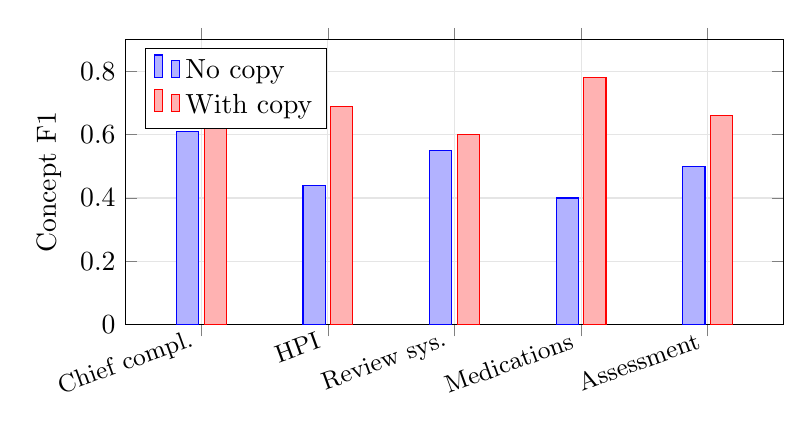
\begin{tikzpicture}
\begin{axis}[
    width=0.82\textwidth, height=5.2cm,
    ybar, bar width=8pt,
    enlarge x limits=0.15,
    ymin=0, ymax=0.9,
    ylabel={Concept F1},
    symbolic x coords={Chief compl., HPI, Review sys., Medications, Assessment},
    xtick=data, x tick label style={rotate=20, anchor=east, font=\small},
    legend pos=north west, legend cell align=left,
    grid=both, grid style={gray!20},
]
\addplot coordinates {(Chief compl.,0.61)(HPI,0.44)(Review sys.,0.55)(Medications,0.40)(Assessment,0.50)};
\addplot coordinates {(Chief compl.,0.74)(HPI,0.69)(Review sys.,0.60)(Medications,0.78)(Assessment,0.66)};
\legend{No copy, With copy}
\end{axis}
\end{tikzpicture}
\caption{Concept F1 by note section. The copy mechanism is most valuable where
patient-specific entities are dense (history of present illness, medications).}
\label{fig:bysection}
\end{figure}

\subsection{Human evaluation}

On a blinded sample of $200$ generated drafts, clinicians rated $63\%$ as usable with
only minor edits, $28\%$ as requiring major edits, and $9\%$ as not usable.
Inter-rater agreement was substantial ($\kappa = 0.68$). The rate of drafts needing
only minor edits is the quantity most predictive of whether the tool would save time
in practice, since those are the drafts a clinician can accept with a quick pass.

\subsection{Error analysis}

We examined the drafts rated not usable and the concept-level false negatives. Errors
of \emph{omission} dominate: the model most often fails on facts that were stated only
implicitly or established across several dialogue turns (for example, a symptom's
duration assembled from a back-and-forth exchange), which the attention---anchored on
local lexical matches---does not aggregate. Errors of \emph{commission}, such as
copying a drug the patient mentioned they had \emph{stopped}, are rarer but more
dangerous, and stem from the model copying an entity without its surrounding
negation or temporal qualifier. These patterns suggest that discourse-level modeling
of negation and temporality, rather than more fluent generation, is the productive
next direction.

\section{Discussion and Limitations}

Our results indicate that draft clinical notes can be generated from conversation at
a quality that clinicians find largely edit-ready, and that a copy mechanism is the
component that makes the clinically critical tokens reliable.

\paragraph{Where the clinical value lies.} Documentation is among the largest
non-clinical demands on physician time and a documented driver of burnout, so the
relevant question is not fluency for its own sake but whether the draft shifts the
clinician from \emph{authoring} to \emph{reviewing}. Two of our findings speak to
that shift. First, the $63\%$ of drafts rated usable with only minor edits are
exactly those a clinician can accept with a quick verifying pass rather than rewrite,
and it is this fraction---not the ROUGE score---that determines whether time is
actually saved. Second, the value concentrates in the history of present illness and
the medication list (Figure~\ref{fig:bysection}), the sections that are most
patient-specific and therefore most tedious to compose by hand and least amenable to
static templates; these are precisely where copying helps most. The concept-level F1
we report is not merely an alternative metric but a safety-relevant one: a note that
reads well but records the wrong drug or dose is worse than no draft, so a metric
that tracks whether the right clinical facts survive is the one a deployment should be
governed by. The gain from $0.52$ to $0.71$ in concept F1 is thus the result with the
most direct bearing on clinical utility. Several caveats apply.
We assume clean transcripts; real deployments must contend with speech-recognition
error, which will degrade exactly the rare terms copying depends on. The corpus is
single-institution and English, and documentation style varies across clinicians and
specialties. Most importantly, a generated note that reads fluently can still be
wrong in ways a hurried reviewer may miss, so any deployment must keep the clinician
firmly in the loop and should surface the model's uncertainty and its copy
provenance to support verification.

\section{Conclusion}

We presented an attentional sequence-to-sequence model with a copy mechanism for
generating clinical notes from doctor--patient conversations, and showed that copying
is decisive for rendering the rare medical entities on which clinical correctness
hinges, lifting concept-level F1 from $0.52$ to $0.71$ and producing drafts that
clinicians largely judged edit-ready. The remaining errors are concentrated in
implicit and negated information, pointing toward discourse-aware modeling as the
next step.

\subsubsection*{Acknowledgments}

We thank participating clinicians for annotation and blinded review, and the clinical
informatics team for transcript de-identification.

\small
\begin{thebibliography}{99}

\bibitem{Aronson2010}
A.~R. Aronson and F.-M. Lang.
\newblock An overview of MetaMap: historical perspective and recent advances.
\newblock \emph{Journal of the American Medical Informatics Association},
17(3):229--236, 2010.

\bibitem{Bahdanau2015}
D.~Bahdanau, K.~Cho, and Y.~Bengio.
\newblock Neural machine translation by jointly learning to align and translate.
\newblock In \emph{International Conference on Learning Representations (ICLR)}, 2015.

\bibitem{Cho2014}
K.~Cho, B.~van Merri\"enboer, C.~Gulcehre, et al.
\newblock Learning phrase representations using RNN encoder--decoder for statistical
machine translation.
\newblock In \emph{Proc.\ EMNLP}, 2014.

\bibitem{Graves2005}
A.~Graves and J.~Schmidhuber.
\newblock Framewise phoneme classification with bidirectional LSTM and other neural
network architectures.
\newblock \emph{Neural Networks}, 18(5--6):602--610, 2005.

\bibitem{Gu2016}
J.~Gu, Z.~Lu, H.~Li, and V.~O.~K. Li.
\newblock Incorporating copying mechanism in sequence-to-sequence learning.
\newblock In \emph{Proc.\ ACL}, 2016.

\bibitem{Gulcehre2016}
C.~Gulcehre, S.~Ahn, R.~Nallapati, B.~Zhou, and Y.~Bengio.
\newblock Pointing the unknown words.
\newblock In \emph{Proc.\ ACL}, 2016.

\bibitem{Hochreiter1997}
S.~Hochreiter and J.~Schmidhuber.
\newblock Long short-term memory.
\newblock \emph{Neural Computation}, 9(8):1735--1780, 1997.

\bibitem{Lin2004}
C.-Y. Lin.
\newblock ROUGE: A package for automatic evaluation of summaries.
\newblock In \emph{Text Summarization Branches Out (ACL Workshop)}, 2004.

\bibitem{Mikolov2013}
T.~Mikolov, I.~Sutskever, K.~Chen, G.~Corrado, and J.~Dean.
\newblock Distributed representations of words and phrases and their compositionality.
\newblock In \emph{Advances in Neural Information Processing Systems (NIPS)}, 2013.

\bibitem{Nallapati2016}
R.~Nallapati, B.~Zhou, C.~dos Santos, C.~Gulcehre, and B.~Xiang.
\newblock Abstractive text summarization using sequence-to-sequence RNNs and beyond.
\newblock In \emph{Proc.\ CoNLL}, 2016.

\bibitem{Papineni2002}
K.~Papineni, S.~Roukos, T.~Ward, and W.-J. Zhu.
\newblock BLEU: a method for automatic evaluation of machine translation.
\newblock In \emph{Proc.\ ACL}, 2002.

\bibitem{Rush2015}
A.~M. Rush, S.~Chopra, and J.~Weston.
\newblock A neural attention model for abstractive sentence summarization.
\newblock In \emph{Proc.\ EMNLP}, 2015.

\bibitem{Sutskever2014}
I.~Sutskever, O.~Vinyals, and Q.~V. Le.
\newblock Sequence to sequence learning with neural networks.
\newblock In \emph{Advances in Neural Information Processing Systems (NIPS)}, 2014.

\bibitem{Uzuner2011}
\"O. Uzuner, B.~R. South, S.~Shen, and S.~L. DuVall.
\newblock 2010 i2b2/VA challenge on concepts, assertions, and relations in clinical
text.
\newblock \emph{Journal of the American Medical Informatics Association},
18(5):552--556, 2011.

\bibitem{Vinyals2015}
O.~Vinyals, M.~Fortunato, and N.~Jaitly.
\newblock Pointer networks.
\newblock In \emph{Advances in Neural Information Processing Systems (NIPS)}, 2015.

\end{thebibliography}

\end{document}
